\chapter{Search and learning}
\label{ch:search}

The planner of the previous chapters makes many choices with quick
estimates: the direction of the passes from their length and number, the
order of the cells from estimated transfers. This last chapter asks how
good these estimates are, and what can be gained by replacing them, either
by planning every option and keeping the best (\emph{search}), or by a model
learned from many planned examples (\emph{learning}). It ends with what the
course leaves open.

\section{How good is the estimate?}

The estimate of Chapter~\ref{ch:swaths} counts the length of the passes at
mowing speed and one standard turn per pass. A planned cell differs in
three ways: the ends of the passes are oblique, so the turns join passes
whose ends are not side by side; a turn that does not fit is replaced by a
slower one, or the passes are shortened; and short passes cost a whole
turn for little grass.

To measure the difference, the code draws random convex cells (four to
seven points on an ellipse with half-axes of 3 to \SI{10}{\metre}),
surrounds each with a border of \SI{2.02}{\metre} (the depth of two headland
passes, so that the turns have the room they would have inside a lawn),
picks a candidate direction, and plans the cell with the planner of
Chapter~\ref{ch:swaths}.

On 100 such cells, the estimate is \SI{2.7}{\percent} off the planned time
on average, and up to \SI{13}{\percent}; it is almost always too low (it
ignores the slower turns at oblique ends and the passes shortened to make a
turn fit). What matters for the planner, however, is not the time itself
but which direction it picks. For 60 random cells, the code plans every
candidate direction in which the cell is monotone, and compares the best
with the one the estimate picks: the estimate picks the best direction for
48 cells, and on average costs \SI{0.50}{\percent} more than the best
(\SI{8.6}{\percent} in the worst cell). An estimate can be off by several
percent and still rank the options well, because its errors are similar for
all the directions of a cell.

\section{Search}

The direct answer to an imperfect estimate is not to estimate: plan the
cell in every candidate direction and keep the fastest. Each plan of a cell
takes a fraction of a second here, so for a few cells and a dozen
directions, search is affordable; for many more choices made together (the
decomposition, the directions and the order of the cells), the number of
combinations grows too fast to plan them all, and the estimates come back
as the way to prune them.

On the example lawns, search changes nothing: planning every candidate
direction of each cell of the L-shape and of the garden (with the lawn's
own border, and the lateral order of the passes) picks the directions the
estimate had picked, $0°$ and $90°$ for the two cells of the L-shape, $0°$
and $12°$ for the cells of the garden, and the plans are the same
(\SI{9.02}{\minute} and \SI{15.96}{\minute}). Their cells are close to
rectangles, where the estimate is at its best; the random cells above,
with their oblique sides, are where it errs.

\section{Learning a better estimate}

Between the two, a model can learn from planned examples to predict the
time of a cell, and replace the estimate where the planner needs a number
quickly. The features are simple quantities of the swaths: the estimate
itself, the number of passes, their total length, the sum of the jumps of
their ends from one pass to the next, the number of passes shorter than
\SI{2}{\metre}, and the average jump per pass relative to the spacing (how
oblique the ends are). The model is linear,
\[
  \hat t = w_0 + \sum_{i=1}^{6} w_i f_i ,
\]
fitted by least squares (with a little ridge regularisation, after scaling
each feature) on 400 planned examples and tested on 100 others.

The learned model is off by \SI{1.45}{\percent} on average on the test
cells (\SI{7.4}{\percent} at most), against \SI{2.7}{\percent} for the
estimate alone. Its largest weights say what the estimate misses: about
$w_2 = \SI{6.7}{\second}$ per pass on top of a reduced share of the
estimate, the cost of a turn that is longer than the standard one. Used to
choose the directions of the same 60 cells, it picks the best direction for
53 cells instead of 48, and costs \SI{0.33}{\percent} more than the best on
average instead of \SI{0.50}{\percent}; the worst cell is the same, at
\SI{8.6}{\percent}, a direction that neither predicts.

\begin{figure}[ht]
  \centering
  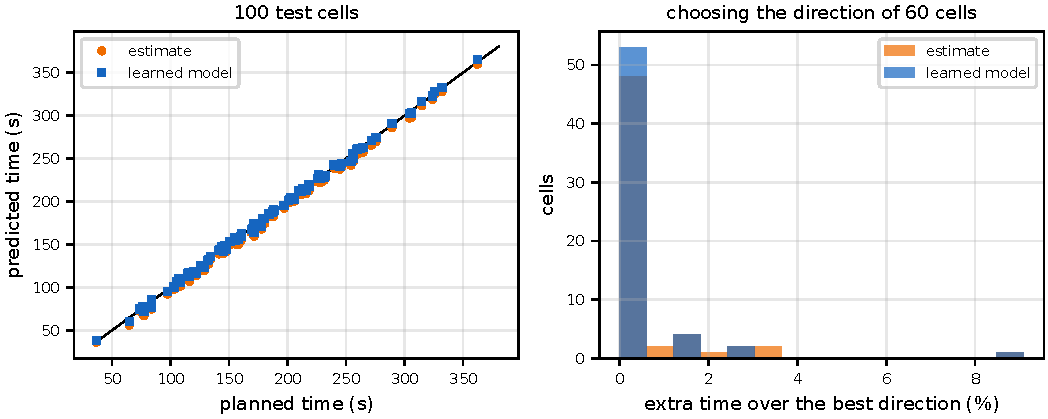
\includegraphics[width=\textwidth]{figures/learning}
  \caption{Left: the time predicted by the estimate (orange) and by the
    learned model (blue) against the planned time, for 100 random cells not
    used to fit the model; the black line is a perfect prediction. Right:
    for 60 other random cells, the extra time of the direction chosen by the
    estimate and by the model, compared with the best direction found by
    planning them all; most choices are the best (0\,\%).}
  \label{fig:learning}
\end{figure}


\section{Learning the whole plan?}

The project this course grew from tried another route: learn the whole
path, cell by cell on a grid, with reinforcement learning and Monte Carlo
tree search. On a real lawn with a car-like mower, the experience of these
chapters suggests where learning fits best. The geometry (offsets, swaths,
the shortest paths of a car) has exact answers, and the planner computes
them reliably; a learned policy would have to rediscover them, and would
give no guarantee that the mower stays on the lawn. What remains are the
choices made with estimates: the cuts, the directions, the order, the
pattern of the passes. These are few, discrete, and each can be evaluated
by planning, which is the setting where search (Monte Carlo tree search
among them) and learned estimates do well: learning proposes, the planner
checks.

\section{What is left}

\begin{description}
  \item[Variable clearance.]
    \leavevmode\\
    The first headland pass keeps the same clearance all along; a clearance
    that grows only where the swing-out needs it would leave less uncut.
  \item[Continuous-curvature paths.]
    \leavevmode\\
    The turns with ramps of Chapter~\ref{ch:smooth} are adjusted from
    Reeds--Shepp paths; the exact shortest paths with bounded curvature rate
    (Fraichard and Scheuer) would be faster.
  \item[Coverage as a goal.]
    \leavevmode\\
    The planner aims at covering the lawn and measures the result; it could
    instead target the gaps that remain (the corners, the strip along the
    border) with short extra passes.
  \item[The real world.]
    \leavevmode\\
    Slopes, wet grass that makes the wheels slip, the side where the deck
    throws the grass, a fuel tank or a battery, people and animals crossing
    the lawn: each changes the model or the plan, and each can be added to
    the simulator in the same way, measured by the same function.
\end{description}

\begin{inwords}
  Quick estimates are good enough for most choices, and planning every
  option is the surest improvement where it is affordable. A model learned
  from plans sits between the two. Learning is most useful here not to
  replace the geometry, which has exact answers, but to make the few
  high-level choices faster.
\end{inwords}

\begin{incode}
  \code{mowersim/planning/learn.py}: \code{random\_cell}, \code{features},
  \code{cell\_time}, \code{dataset}, \code{fit} (the linear model),
  \code{choose\_direction} (by estimate, model or search) and
  \code{regret\_study}; \code{plan(..., directions="search")} in
  \code{mowersim/planning/planner.py}. From the command line:
  \begin{verbatim}
python -m mowersim plan lawns/garden.json --directions search
  \end{verbatim}
\end{incode}
